\documentclass[conference]{IEEEtran}
% Supplementary material for main_sc.tex (the SC-length paper); main_v2.tex is the full-length version.
% Build: paper/build.sh supplement
% Figures: gh200/analysis/paper_figures.py and mi350/analysis/paper_figures_mi350.py -> figs/
\usepackage{cite}
\usepackage{amsmath}
% Times-compatible fonts under XeTeX (IEEEtran's ptm Times is not available in the TU encoding tectonic uses)
\usepackage{fontspec}
\setmainfont{texgyretermes}[Extension=.otf,UprightFont=*-regular,BoldFont=*-bold,ItalicFont=*-italic,BoldItalicFont=*-bolditalic]
\setsansfont{texgyreheros}[Extension=.otf,UprightFont=*-regular,BoldFont=*-bold,ItalicFont=*-italic,BoldItalicFont=*-bolditalic]
\setmonofont{texgyrecursor}[Extension=.otf,UprightFont=*-regular,BoldFont=*-bold,ItalicFont=*-italic,BoldItalicFont=*-bolditalic]
\usepackage{unicode-math}
\setmathfont{texgyretermes-math.otf}
\usepackage{graphicx}
\usepackage{booktabs}
\usepackage{multirow}
\usepackage{url}
\usepackage{xcolor}
\usepackage[hidelinks]{hyperref}

\newcommand{\W}{\,W}
\newcommand{\Eh}{\,E$_\mathrm{h}$}
\newcommand{\Ry}{\,Ry}
\newcommand{\ee}[2]{#1{\times}10^{#2}}  % \ee{1.2}{-5} -> 1.2x10^-5 (math mode)
\newcommand{\pct}{\%}
% Results of experiments still running when this draft was written; every occurrence must be gone before submission.
\newcommand{\pending}[1]{\textcolor{red}{[pending: #1]}}

\begin{document}
\bstctlcite{IEEEexample:BSTcontrol}
\renewcommand{\thetable}{S\arabic{table}}
\renewcommand{\thefigure}{S\arabic{figure}}
\renewcommand{\thesection}{S\arabic{section}}

\title{Supplementary Material: Switching-Aware Precision Selection on Power-Capped GPUs}
\author{\IEEEauthorblockN{Anonymous}}
\maketitle

This supplement collects measurements that support, but are not needed for, the conclusions of the paper: results
obtained through the GH200 interposer (upper bounds), third-party non-GEMM codes, single-precision replacements, the
GH200 emulation shape sweep, further Gaussian-process experiments, the GH200 HPL tuning, and the AI workloads. Section
references of the form ``Section~III'' point to the paper.

\section{Interposer Results on GH200 (Upper Bounds)}\label{sec:sci}

Plane-wave DFT is tolerant. With 28 kept bits, the total energies of QE Si\,1000 and Au\,112 move by
$\ee{1.0}{-5}$ and $\ee{2.3}{-5}$\Ry{} under truncation and by $\ee{3.5}{-7}$ and $\ee{2.8}{-7}$\Ry{} under
round-to-nearest. The gold surface still converges at 20 bits with nearest rounding ($\ee{5.5}{-5}$\Ry, both runs);
for Si\,1000, 20 bits is the failure edge (one run converges with $\ee{1.1}{-4}$\Ry, the other aborts at iteration
24), and truncation diverges or slows at 20 bits. Gaussian-basis quantum chemistry needs more bits. GPU4PySCF
valinomycin DFT errs by $\ee{1.1}{-8}$\Eh{} at 44 bits; at 36 bits the energy oscillates near $10^{-8}$\Eh{} and
cannot meet a $10^{-10}$ convergence threshold, but with the chemically sufficient $10^{-7}$ threshold 40, 36 and 32
bits converge in the same 12 iterations as native, with a 32-bit nearest error of $\ee{1.2}{-5}$\Eh{}
($\approx$0.007\,kcal/mol). At 36--40 bits the error is then set mainly by the threshold (32 bits errs an order of
magnitude more), consistent with the $\approx$37 significant bits found sufficient by Dawson et
al.~\cite{Dawson2024}.

Under caps, with the shim truncating every GEMM and compared against a baseline that takes the same copy path
without truncating, Si\,1000 at 550\W{} with 28-bit nearest rounding is 6.2\pct{} faster and uses 6.4\pct{} less
energy (SM clock 1348$\to$1446\,MHz), and Au\,112 at 450\W{} is 4.9\pct{} faster with 5.1\pct{} less energy (one
truncated run each, between baseline runs before and after).
These are upper bounds for a library that truncated internally; against the unmodified program the shim is
0.4\pct{} slower (Au\,112, 450\W) because of its $\approx$5\pct{} copy cost. The in-program version of
Section~VI-C truncates only Davidson blocks without copies and is the deployable number.

For GPU4PySCF, nsys shows FP64 GEMM kernels at 46\pct{} of GPU kernel time and 32\pct{} of total runtime for
valinomycin DFT (31\pct{} and 27\pct{} of kernel time for taxol and tamoxifen); the rest is dominated by copies of
computed intermediates (36--50\pct) and integrals. With 32--36 bits needed and FP64 GEMM keeping 35 bits
5.1--6.5\pct{} faster at 500--800\W, truncation alone is bounded at about $32\pct\times5$--$6.5\pct\approx1.6$--2.1\pct{}
end to end (3.9\pct{} at 400\W). This estimate assumes the default grid and GEMM time proportional to flops at
1000\W{} speed; on a finer grid (level 6), valinomycin measured at 450--550\W{} is 3.3--3.5\pct{} faster
(Section~VII-B). Neither number implies that truncation beats INT8 emulation here: the two
dominant GEMM shapes favor different methods (Section~VII-A), and choosing by shape bounds the gain at
about 3.5\pct{} with cuBLAS emulation for the long-$k$ shape, or 6.6\pct{} with the less accurate GEMMul8.

\textbf{Wide range, partly power-bound DFT.} These DFT runs draw only 650--690\W{} at 1000\W, but are power-bound
below that. For valinomycin (grid level 6) at 550 and 450\W, rounding to 36 bits through the shim is 3.3--3.5\pct{}
faster than the copy baseline with 2--3\pct{} less energy and an error of $\ee{9.5}{-7}$\Eh; emulation must keep 40
bits to stay correct, which is then about ten times more accurate ($\ee{8.4}{-8}$\Eh) but takes 1.48--1.53$\times$
the baseline time (two rounds each).

\textbf{ExaGeoStat itself (GH200).} We also built ExaGeoStatCPP (StarPU and Chameleon tile Cholesky with cuBLAS~13.6; tile
size 1920) and ran its MLE ($N=60000$, six BOBYQA likelihood evaluations per run, data generated once natively and
read by every run) with the shim on its FP64 tile GEMMs. Matérn covariance generation runs on the CPU and takes about
9\,s per evaluation against 2.3\,s of GPU factorization at 1000\W, and the factorization is partly power-limited even
there (GPU power about 620--670\W{} on average, frequent power-cap events). Relative to a baseline that copies the operands without
truncating, the factorization is 3.0\pct{} (36 bits) and 4.0\pct{} (28 bits) faster at 1000\W, 5.0\pct{} and
8.0\pct{} at 600\W, and 5.6\pct{} and 9.4\pct{} at 450\W{} (means of two ABBA rounds; at 450\W{} the rounds differ
widely, +6.9 and +11.9\pct{} with 28 bits at 707 and 926\,MHz, because the CPU shares the module cap while generating
the covariance); with 28 bits the mean SM clock during factorization rises from 1913 to 1975\,MHz at 1000\W{} and
from 1166 to 1305\,MHz at 600\W. The log-likelihoods change by at most $\ee{1.2}{-10}$ and $\ee{9.8}{-8}$ relative.
The shim's own copy costs 7--9\pct, which leaves it 0.5--3.1\pct{} slower than unmodified ExaGeoStat, so the gain
needs an implementation inside the library. ExaGeoStatCPP's mixed-precision option (\texttt{-{}-computation=mixed}) is
only an enumeration value without an implementation, so we could not compare with its own mixed precision.

\begin{figure}[t]
\centering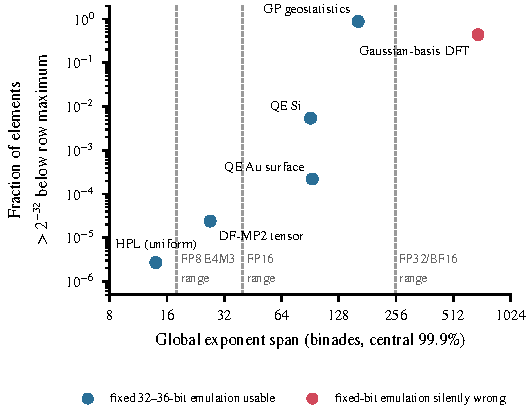
\includegraphics[width=\columnwidth]{figs/range_map.pdf}
\caption{GH200: global exponent span (central 99.9\pct) against the flop-weighted fraction of elements more than $2^{-32}$
below their row maximum, with the measured outcome of fixed 32--36-bit cuBLAS emulation (e.g., HPL: residual 0.197,
passes; Gaussian-basis DFT: 52.5\,mE$_\mathrm{h}$ error; Gaussian process: global span 162, estimate unchanged). All
points are measured; coordinates and their sources are listed in
\texttt{gh200/results/range\_map\_points.csv}.}\label{fig:map}
\end{figure}

Fig.~\ref{fig:map} places the measured codes by their global exponent span and the flop-weighted fraction of
elements far below their row maximum, with the outcome of fixed-width cuBLAS emulation on each (paper, Section~VII-B).

\section{Third-Party Non-GEMM Codes (GH200)}\label{sec:thirdparty}
\textbf{Third-party codes (GH200).} We zeroed, once at setup, the coefficient arrays that are stored and multiplied in every
step in three GPU FP64 codes: MFEM's partial-assembly quadrature data (about 43\pct{} of CG memory traffic), SW4's
material parameters (about 9\pct) and LAMMPS EAM tables (cache resident). Without zeroing all three are bitwise
identical to the originals or within rerun noise. MFEM (38.27\,M unknowns, $p=3$) is 0.9/2.0\pct{} faster with
36/20 bits (nearest) at 450\W{} and 0.7/1.4\pct{} at 550\W, unchanged at 1000\W; the solution changes by at most
$\ee{2.3}{-11}$. SW4 (123\,M grid points) is 0.6/1.3\pct{} faster at 350\W{} and 0.3/0.5\pct{} at 450\W{}, with
receiver waveforms changing by at most $\ee{3.4}{-11}$/$\ee{3.4}{-6}$ (doubling the grid changes them by 4--10\pct);
LAMMPS EAM (16.38\,M atoms) moves 0.0--0.4\pct, within noise. The gain order, MFEM $\ge$ SW4 $>$ LAMMPS, follows
the coefficients' share of memory traffic: kernel-level gains of 4.8--14.0\pct{} at 450--500\W{} are diluted by the rest of the
full-mantissa computation. Zeroing fits best when inputs flow directly and in volume into multipliers or data
paths.

\section{FP32 and 3xTF32: Accumulation, Not Range (GH200)}\label{sec:fp32}

3xTF32 (our own implementation, in the shim and in a benchmark script, not the CUTLASS one) is the fastest method in
Table~\ref{tab:methods} but has only FP32-level accuracy, and its error grows with the inner dimension: on $4096{\times}4096$ it is $\ee{6.4}{-7}$, $\ee{4.8}{-6}$ and $\ee{3.8}{-5}$ at $k=256$, 2048 and
16384, whereas FP32 SGEMM grows as $\sqrt{k}$ ($\ee{2.9}{-7}$, $\ee{8.1}{-7}$, $\ee{2.3}{-6}$) and FP64 truncation
is independent of $k$. The measured log slope of about one (7.5--7.9$\times$ per 8$\times$ in $k$) points to a
systematic error in TF32 tensor-core accumulation rather than random rounding, consistent with the round-toward-zero
accumulation Fasi et al.\ found on V100, T4 and A100~\cite{Fasi2021} (bit-accurate Hopper models:~\cite{Khattak2025}).
At $k=2048$ its error is 18 times that of FP64 rounded to nearest at 20 bits ($\ee{2.6}{-7}$) and 7 times that of
FP64 truncated to 20 bits ($\ee{6.7}{-7}$).

Quantum ESPRESSO's operands fit in FP32's range, so we replaced every FP64 and complex FP64 GEMM with single
precision through the shim (inputs to FP32; 3xTF32 additionally splits into big and small parts multiplied three
times on TF32 tensor cores; $C$ combined in FP64). On the gold surface at 450\W{} (2 interleaved runs each), FP32
aborts at SCF iteration 26 and 3xTF32 and TF32 at iteration 2 when the Davidson bands fail to converge, and the
integrated charge drifts from 1232 electrons (FP32 $+0.012$, 3xTF32 $+0.074$); FP64 rounded to 24 and 20 bits
differs from native by $\ee{8.1}{-6}$ and $\ee{5.5}{-5}$\Ry{} and converges in 28 iterations. Si\,1000 at 550\W{}
behaves the same: FP32 aborts at iteration 14 and 3xTF32 at 9, with 4000.18 and 4001.52 electrons instead of 4000.
The difference is accumulation: truncated FP64 still accumulates in FP64, while Quantum ESPRESSO's inner dimension
is the number of plane waves (95386 on the gold surface plus a real GEMM with $k=4.3{\times}10^{6}$; 375286 for
Si\,1000), where 3xTF32 already errs by $\ee{5.6}{-5}$ to $\ee{2.2}{-4}$, the same order as plain TF32. FP32 GEMM on
Hopper is also slower than FP64 tensor cores (on the gold surface about 1.5$\times$ per SCF iteration, estimated).
Replacing every GEMM with single precision thus fails for this long-inner-product solver even though the range fits;
mixed precision that uses FP32 only in selected steps, as Woo et al.\ do~\cite{Woo2023}, is a different matter. FP64
truncation is the reduced-precision choice here that leaves the algorithm unchanged.

\section{Emulation Crossover on GH200: Shapes, Caps and a Model}\label{sec:gh200xover}
\begin{table}[t]
\caption{GH200: the two GEMM shapes that each carry 35\pct{} of valinomycin DFT flops: tall-skinny
$757248{\times}300{\times}2958$ and long-$k$ $2958{\times}2958{\times}76800$ (TFLOP/s; relative error in parentheses;
GEMMul8 errs by $\ee{1.0}{-10}$ and $\ee{8.2}{-10}$ on the two shapes, 10--80 times more than truncation to 36
bits).}\label{tab:shape}
\centering\footnotesize\setlength{\tabcolsep}{4pt}
\begin{tabular}{@{}lrrrr@{}}
\toprule
& \multicolumn{2}{c}{Tall-skinny} & \multicolumn{2}{c}{Long $k$} \\
\cmidrule(lr){2-3}\cmidrule(l){4-5}
Method & 1000\W & 575\W & 1000\W & 575\W \\
\midrule
FP64 native & 51.6 & 36.8 & 50.6 & 36.2 \\
Truncation, 36 bits ($\ee{1.0}{-11}$) & 54.0 & 38.9 & 53.7 & 38.0 \\
cuBLAS emu., 32 bits ($\ee{9.7}{-12}$) & 19.5 & 16.6 & 65.4 & 46.0 \\
cuBLAS emu., 28 bits ($\ee{2.3}{-9}$) & 24.2 & 20.9 & 89.9 & 65.6 \\
GEMMul8, 10 moduli & 17.9 & 16.7 & 102 & 75.6 \\
\bottomrule
\end{tabular}
\end{table}

\textbf{The crossover depends on shape.} Intercepting all 45,574 GEMMs of the valinomycin DFT run on GH200 reveals two
shapes that each carry 35\pct{} of the flops (Table~\ref{tab:shape}). With $n=300$, emulation cannot amortize its
splitting and scaling: even at 28 bits it runs at 0.47--0.57$\times$ native speed, and truncation wins at every
accuracy. With $k=76800$ the fixed costs amortize: emulation is still 21--22\pct{} faster than truncation at the
$10^{-11}$ level, and GEMMul8 is nearly twice as fast at $10^{-9}$. Within one application the best choice is per call:
truncation for tall-skinny shapes, emulation for long $k$.

\begin{figure*}[t]
\centering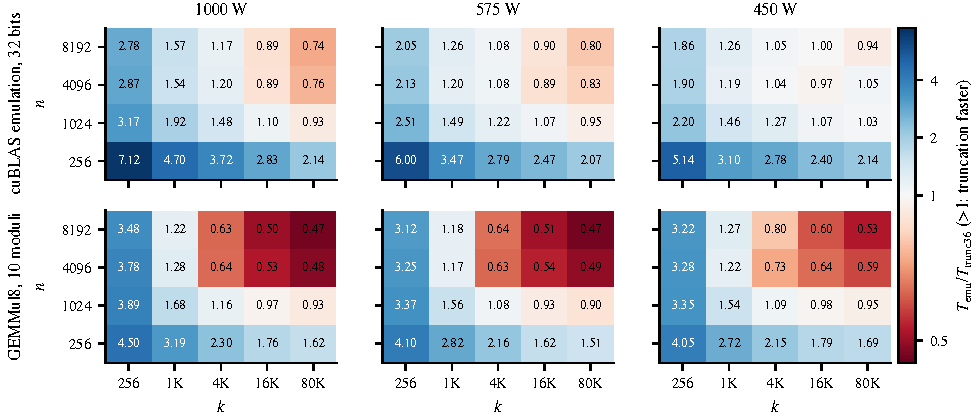
\includegraphics[width=\textwidth]{figs/crossover.pdf}
\caption{GH200: time of INT8 emulation relative to truncation to 36 bits, $T_\mathrm{emu}/T_\mathrm{trunc36}$
($m=8192$; blue: truncation faster). Top: cuBLAS emulation with 32 bits (error comparable to truncation,
$\approx10^{-11}$); bottom: GEMMul8 with 10 moduli (about ten times larger error, $\approx10^{-10}$); columns: module
caps. Means of two rounds.}\label{fig:crossover}
\end{figure*}

\textbf{A shape sweep and a predictive model (GH200).} We fixed $m=8192$ and swept $n\in\{256,1024,4096,8192\}$ and
$k\in\{256,1024,4096,16384,81920\}$ at 1000, 575 and 450\W, two rounds each (480 records; Fig.~\ref{fig:crossover}).
Truncation to 36 bits beat native in all 60 shape--cap combinations (3.8--11.9\pct{} at 450\W, 3.6--5.9\pct{} at
575\W, 0.5--4.8\pct{} at 1000\W). cuBLAS emulation with 32 bits wins roughly when $n\ge4096$ and $k\ge16384$ (and at
$n=1024$, $k=81920$ at 1000 and 575\W) (at best 0.74$\times$ truncation time at 1000\W), and its winning region shrinks at
lower caps: 5 of 20 shapes at 1000 and 575\W, 2 at 450\W. Where the emulation itself is not power-bound, however, lower
caps favor it: at $n=8192$, $k=4096$ its time relative to truncation falls from 1.17 to 1.08 to 1.05 as the cap goes from
1000 to 575 to 450\W. The four values of $n$ were measured on different nodes: each ratio is paired on one node, but
shape effects and node differences cannot be separated. GEMMul8 with 10 moduli needs only 0.47--0.80$\times$ the
truncation time when $n,k\ge4096$, at an order of magnitude larger error ($\approx10^{-10}$ versus $10^{-11}$), and is up
to 4.5$\times$ slower when $n$ or $k$ is small. Emulation's extra work is input splitting ($\propto mk+nk$) and output
accumulation ($\propto mn$); dividing by the $mnk$ multiply gives
\begin{equation}
T_\mathrm{emu}/T_\mathrm{trunc} = A + B\,(1/m + 1/n) + C/k,
\end{equation}
where $A$ is the ratio of per-flop speeds. Least-squares fits per cap (about 20 points for three parameters, so $R^2$ is
only descriptive) reach $R^2=0.98$--0.99 for GEMMul8, versus 0.86--0.89 for a single effective size
$1/(1/m+1/n+1/k)$; cuBLAS emulation reaches only 0.88--0.89. On the two held-out valinomycin shapes the model picks the
winner in 8 of 8 cases, all far from the crossover, so this is a loose test; the model is an empirical description of
these measurements.

\begin{table}[t]
\caption{GH200: square GEMM ($32768{\times}32768{\times}2048$) in TFLOP/s by cap on one node, native FP64 first and the
other methods ordered by relative error.}\label{tab:methods}
\centering\footnotesize\setlength{\tabcolsep}{4pt}
\begin{tabular}{@{}lrrr@{}}
\toprule
Method (error) & 1000\W & 575\W & 450\W \\
\midrule
FP64 native & 59.2 & 43.2 & 35.8 \\
Trunc., 36 bits ($\ee{1.0}{-11}$) & 61.8 & 45.5 & 38.6 \\
GEMMul8, 10 moduli ($\ee{1.0}{-10}$) & 70.8 & 51.4 & 34.7 \\
GEMMul8, 9 moduli ($\ee{1.6}{-9}$) & 78.2 & 56.6 & 38.2 \\
cuBLAS emu., 28 bits ($\ee{2.3}{-9}$) & 67.8 & 55.2 & 47.5 \\
Trunc., 28 bits ($\ee{2.6}{-9}$) & 63.2 & 46.6 & 39.6 \\
FP32 SGEMM ($\ee{8.1}{-7}$) & 51.2 & 40.4 & 34.6 \\
3xTF32 ($\ee{4.8}{-6}$) & 96.6 & 72.0 & 56.4 \\
\bottomrule
\end{tabular}
\end{table}

\textbf{The power of the emulation itself changes the winner.} On GH200, GEMMul8 draws about 970\W{} at a 1000\W{} cap and at
450\W{} its clock drops to 650--720\,MHz, where truncation becomes faster; cuBLAS fixed-point emulation with 28 bits draws only
about 706\W{} at 1000\W{} and gains relative ground at lower caps on the square shape (Table~\ref{tab:methods}).
Which way a tighter cap tips the balance thus depends on how much power the emulation itself draws.

\section{Gaussian Process: Maximum-Likelihood Fit and Tile Mixed Precision (GH200)}\label{sec:gpextra}
\textbf{A one-parameter maximum-likelihood fit (GH200).} To check that the estimate itself is unchanged, we fitted the range
parameter with variance and smoothness fixed: golden-section search over its logarithm, 17 likelihood evaluations
per variant ($n=60000$; 1000 and 700\W; two interleaved rounds). Truncation to 36 and 28 bits and cuBLAS emulation
return the native estimate
$\hat\theta=0.05007952$ in every printed digit, with maximized log-likelihoods within $\ee{4.8}{-6}$ (36 bits) and
$\ee{2.3}{-4}$ (28 bits) of native; FP32 moves $\hat\theta$ by 0.49\pct{} and loses 0.72 in log-likelihood. At
700\W{} the fit is 7.1--7.3\pct{} faster with 28 bits
and 4.8--4.9\pct{} faster with 36 bits, using 6.6--6.8\pct{} and 4.5--4.8\pct{} less energy; at 1000\W{} it is
1.8--2.3\pct{} and 1.6--2.2\pct{} faster with 9.1--9.9\pct{} and 3.5--5.6\pct{} less energy; cuBLAS emulation is
32--41\pct{} slower. Of the three whole-matrix choices we tested (FP32, 36-bit cuBLAS emulation and truncation), only
truncation is both fast and accurate on this wide-range, power-bound workload.

\textbf{Composing with tile mixed precision (GH200).} The mixed-precision Cholesky factorizations of the ExaGeoStat line change
the format of whole tiles instead (Section~II). To see whether truncation still helps there, we ordered
the locations along a Morton curve and added such a variant to our kernel: in the trailing update, tiles below each
column's FP64 extent, chosen by the tile-norm rule with a required accuracy of $10^{-9}$ as in~\cite{Cao2023}, use FP16
inputs with FP32 accumulation on the tensor cores (52\pct{} of the tiles at range 0.02, 3\pct{} at 0.08). Over the six
ranges ($n=60000$, two ABBA rounds) it runs 1.60--1.63$\times$ faster than native FP64 at 1000, 700 and 500\W, with
log-likelihood deviations up to 0.043. Truncating its remaining FP64 tiles to 28 bits makes it another 1.9\pct{}
faster at 1000\W{} and 7.0\pct{} and 6.1\pct{} faster at 700 and 500\W, with an unchanged deviation, so truncation
composes with format changes rather than competing with them. Zeroing the FP16 operands to 5 mantissa bits as well
added nothing.

\section{HPL Tuning and Node Sets on GH200}\label{sec:hpltune}
\textbf{GH200, 8 nodes.} We first tuned native HPL at 1000\W. The configuration inherited from an H200 study ($N=262144$, NB 1024,
$2\times4$, default NCCL) gave 374.8--376.0\,TFLOP/s; fixing NCCL at 8 channels with 2\,MiB buffers (+4.5\pct) and
raising $N$ to 286720 (+2\pct) gave 390.2--398.8\,TFLOP/s in three runs, and no neighboring setting of $N$, NB, split
fraction or NCCL parameters beat this ${\approx}2\pct$ run-to-run spread (24 settings, 26 runs; $f=0.15$ and
$4\times2$ grids were about 2 and 13\pct{} slower). We then swept the caps with this configuration on two node sets: set
A (work4--11) with two ABBA pairs per cap, and set B (work3--8, 12 and 13), measured a day later after one uncounted
warm-up run, with four pairs per cap. That day the second InfiniBand port of most nodes linked at only 2.5\,Gb/s and
NCCL and MPI routed part of the traffic over it (157\,TFLOP/s on 8 nodes); pinned to the 200\,Gb/s port, set B still
reached only 365.5\,TFLOP/s natively at 1000\W, 7\pct{} below set A, although its SM clock was higher (1961 versus
1936\,MHz), so more of its time went to communication. Differences between the sets thus mix nodes and network state; every
pair is matched within one job.


\begin{table}[t]
\caption{GH200: delivered performance on 8 nodes in TFLOP/s, node set A\,/\,B (means per set). HPL: tuned, $N=286720$;
HPL-MxP: $N=491520$, reportable rate including refinement. The 8 GPUs' FP64 tensor-core peak is about 536\,TFLOP/s
($8\times67$\,TFLOP/s~\cite{NVIDIAGH200}).}\label{tab:hplperf}
\centering\footnotesize\setlength{\tabcolsep}{3pt}
\begin{tabular}{@{}lcccc@{}}
\toprule
& \multicolumn{2}{c}{HPL (FP64)} & \multicolumn{2}{c}{HPL-MxP (BF16 LU)} \\
\cmidrule(lr){2-3}\cmidrule(l){4-5}
Cap & Native & 36 bits & Native & 3 bits \\
\midrule
400\W & 225.0/228.0 & 249.9/249.2 & 2076/1922 & 2340/2128 \\
500\W & 288.0/278.2 & 300.7/291.0 & 2823/2555 & 3007/2692 \\
600\W & 318.0/304.5 & 334.0/318.3 & 3229/2858 & 3310/2922 \\
700\W & 346.2/328.3 & 362.9/341.3 & 3449/3039 & 3519/3094 \\
800\W & 370.8/345.8 & 385.6/356.3 & 3655/3178 & 3720/3229 \\
1000\W & 393.9/365.5 & 409.2/367.5 & ---$^{*}$ & --- \\
\bottomrule
\end{tabular}
\\[2pt]{\scriptsize Set A: work4--11 (HPL), work4--7 and 10--13 (HPL-MxP), 2 pairs per cap; set B: work3--8, 12, 13, 4 pairs.
$^{*}$Native HPL-MxP trips the chassis power brake at 1000\W{} on set A; set B was not run there.}
\end{table}

\section{AI Workloads: Training and Inference (GH200)}\label{sec:ai}
\textbf{FP8 inference and its failures.} FP8 training keeps high-precision master weights with per-tensor
scaling, E4M3 for weights and activations and E5M2 for gradients~\cite{Micikevicius2022}; Gupta et al.\ showed that
rounding decides the fate of low-precision training~\cite{Gupta2015}. The clearest FP8 failure is attention:
FlashAttention-3's FP8 mode drops the VQA-a video-quality score of CogVideoX from 70.2 to 6.5 and of HunyuanVideo from
82.5 to 4.4, and 262k-context retrieval from 7.0 to 0.4, which SageAttention2 repairs inside FP8 by smoothing outliers and using a fixed scale for softmax
probabilities~\cite{Zhang2025}. MLPerf Inference closed division allows any pure, reproducible mathematical
quantization but forbids pruning non-zero weights~\cite{MLPerfInfRules}; mantissa zeroing is the former.


MLPerf Training measures time to target quality (eval loss $\le0.925$ on GovReport for Llama\,2 70B LoRA); a faster
step that needs more samples to converge loses.

\textbf{Training: truncating the FP8 base weights is a negative result.} We truncated only the frozen FP8 base weights
of Llama\,2 70B LoRA (once, after loading); activations, gradients, LoRA weights and updates and per-tensor scaling
follow~\cite{Micikevicius2022}. On 8 nodes with the same seed, native FP8 at 575\W{} reached the target after 3456
samples in 28.34\,min. Keeping 2 bits made each 384 samples only 0.9--1.2\pct{} faster but needed 4224 samples (22\pct{}
slower at 575\W, 19\pct{} at 800\W); 1 bit did not converge (it also lowers the largest representable E4M3 value
from 448 to 384, compressing the top weights by about 14\pct). The eval-loss curve shifts up by 0.006--0.008, while
the train-loss gap varies (with 2 bits $-0.031$ at the first logged step, then $+0.003$ to $+0.017$): truncation
weakens the base model at load time, and a rank-16 adapter does not compensate. A second seed (5678, 800\W) agrees: native 3072 samples in 22.74\,min,
2 bits 4224 samples in 31.56\,min (+39\pct). Across two seeds and four pairs (one at 575\W, three at 800\W), the first evaluation is always
0.008--0.010 higher and convergence takes 2--3 more evaluation intervals. Native convergence differs by one interval
between node sets (3072 versus 3456), so we read this only as evidence that FP8's 3 mantissa bits leave no room. The
rounding mode shows no consistent order (at 800\W{} truncation and stochastic rounding converge at 4224 samples,
nearest at 5376). Truncating only MLP layers needs 4224 samples, attention only 3840 (one interval, within node-set
noise, but attention is only about 18\pct{} of the linear weights); the first-evaluation gaps of $+0.0064$ (MLP) and
$+0.0028$ (attention) roughly add up to the $+0.0086$ of full truncation (their sum is 0.0092). A repeat of the
attention-only run gave nearly the
same first evaluation (0.9428 versus 0.9425) but converged one interval later (4224 versus 3840, missing the target by
$10^{-5}$ at 3840), so the first-evaluation gap, not the convergence point, is the robust metric.

\begin{table}[t]
\caption{WikiText-2 perplexity (sequence 2048) relative to BF16 for the linear layers' formats; FP8 uses real FP8
tensor-core GEMMs, and kept bits are rounded to nearest (ties to even).}\label{tab:llm}
\centering\footnotesize\setlength{\tabcolsep}{2.2pt}
\begin{tabular}{@{}lrrrrrr@{}}
\toprule
Format & L2-7B & L3.1-8B & Qw2.5-7B & Mis-7B & OPT-6.7B & L2-70B \\
\midrule
BF16, 4 b & +0.09 & +0.19 & +0.13 & +0.09 & +0.45 & +0.10 \\
BF16, 3 b & +0.44 & +1.02 & +0.65 & +0.41 & +2.00 & +0.51 \\
FP8 per tensor & +0.63 & +0.95 & +0.70 & +0.45 & +2.23 & +0.48 \\
FP8 per channel & +0.32 & +0.88 & +0.61 & +0.34 & +0.69 & +0.42 \\
FP8 p.c., 2 b & +3.2 & +6.5 & +4.0 & +2.5 & +7.0 & +3.4 \\
FP8, wts.\ 2 b & +1.9 & +4.0 & +2.6 & +1.3 & +2.8 & --- \\
\bottomrule
\end{tabular}
\\[2pt]{\scriptsize Values in percent. b: kept bits; L: Llama, Qw: Qwen, Mis: Mistral; p.c.: per channel; wts.: weights only.}
\end{table}

\textbf{Inference: FP8 has already taken most of the benefit.} BF16 rounded to nearest at 3 bits has as many mantissa
bits as FP8 E4M3 and matches its accuracy on six language models (Table~\ref{tab:llm}; with truncation, 4 bits are
needed for a similar GEMM error, 4.35\pct{} on uniform data). We then compared the two where FP8 is known to fail:
attention perplexity at 2k/8k context (BF16 3 bits +0.49/+1.06\pct, emulated FP8 attention +0.52/+1.08\pct), key
retrieval at 8k--32k context on Llama-3.1-8B (both 100\pct), BERT-large SQuAD (all formats above 99.9\pct{} of FP32
F1) and CogVideoX-2B video generation (PSNR against native 18--38\,dB for FP8 attention, 20--29\,dB for BF16 3 bits).
With proper scaling the two tie, and FP8 GEMMs are about 1.7--1.9$\times$ as fast (at 575\W, 1.67--1.72$\times$
BF16 with 3 bits and 1.80--1.87$\times$ native BF16). A naive FP8 attention that does not scale the softmax probabilities fails as sequences grow (74\pct{}
error at 4096 tokens), and on CogVideoX-2B (about 18k tokens) it changes the composition and adds noise (PSNR
10--12\,dB, SSIM 0.07--0.66) where BF16 with 3 bits keeps 20--21\,dB and SSIM 0.82--0.91. This is a range problem,
not a mantissa problem: the smallest positive E4M3 value, about $2^{-9}$, exceeds the mean attention probability over
18k tokens, while BF16 has 8 exponent bits; correct implementations already fix it inside FP8~\cite{Zhang2025}.

Without switching to 2:4 structured sparsity or INT4 weights, zeroing on top of FP8 is the remaining way to go faster
than FP8 on Hopper, which lacks FP4. On real layer-40 activations and weights of Llama2-70B
($8192{\times}57344{\times}8192$), keeping 2 bits on both sides is 4.4/3.2/5.0/8.2\pct{} faster at
1000/700/575/450\W, weights only 1.3--3.3\pct, but 70B perplexity rises by 3.4\pct. Per-layer sensitivity shows
q/k/v as least sensitive but a small share of the compute (with grouped-query attention, q is about 7.8\pct{} and k
and v about 1\pct{} each), and the MLP layers as most of the compute but more sensitive. FP8's
advantage comes mainly from halving the data path: at 575\W{} BF16 with 3 bits is only 8\pct{} faster than BF16,
while FP8 is 1.8$\times$. Power savings are limited too. Decode (64 tokens) is bandwidth-bound; at 1000\W{} zeroing
leaves its speed unchanged on uniform data, though on real Llama2-70B weights zeroed FP8 is still 2.6--3.0\pct{}
faster at the same clock. FP8 zeroed to 0 bits saves
104\W{} on uniform data but only 61\W{} on real Llama2-70B weights, and truncating weights to 2 or 0 bits saves only
1.5\pct{} or 5.5\pct{} of power at an accuracy cost. Below 575\W{} these savings turn into 2--16\pct{} speedups, and
prefill is power-bound even at 1000\W.

For weights and activations that directly set model quality and have no residual correction, zeroing turns directly
into quality loss, in contrast with solvers such as HPL-MxP and SCF that correct errors. For GPUs without FP8 tensor
cores, or pipelines that must stay in BF16, BF16 with 3--4 kept bits is a nearly lossless option; for FP8 deployments,
zeroing saves only 1.5--5.5\pct{} of power in memory-bound phases, at an accuracy cost.

\begin{table*}[t]
\caption{Where each mechanism and experiment lives in the repository.}\label{tab:artifact}
\centering\footnotesize\setlength{\tabcolsep}{4pt}
\begin{tabular}{@{}p{0.4\textwidth}p{0.56\textwidth}@{}}
\toprule
Path & Content \\
\midrule
\path{gh200/bench/}, \path{mi350/bench/} & mantissa GEMM microbenchmarks (cuBLAS; rocBLAS/hipBLASLt with GEMMul8 hook, transposes, exponent spread) and non-GEMM FP64 kernels \\
\path{gh200/shim/mantshim.cu} & cuBLAS interposer: rounding modes, cuBLAS emulation (fixed and automatic, bit-count log), FP32/3xTF32 replacement, exponent-span statistics \\
\path{rocHPL/src/blas/HPL_quantize_device.cpp} & HPL operand rounding (\path{HPL_QUANT_*_BITS}); the AMD build is branch \path{feat/adaptive-mixed-storage} \\
\path{rocHPL-MxP/src_mi350/hplmxp.h} & HPL-MxP zeroing on BF16 write-back (compile-time \path{MANT_BITS}), same source for both platforms \\
\path{apps/q-e/KS_Solvers/Davidson/} & in-program truncation and the tolerance-driven rule (\path{QE_MANT_ADAPT}) \\
\path{apps/pyscf-inputs/mp2_variants.py}, \path{mi350/apps/mp2_prep.py}, \path{mi350/apps/dfmp2.hip} & DF-MP2 variants on GH200; tensor preparation and HIP contraction on MI350X \\
\path{apps/geostat/gp_mle.py}, \path{mi350/apps/gp_chol.hip} & Gaussian-process likelihood and MLE (CUDA/cupy and HIP) \\
\path{mi350/apps/g8_repro.hip} & minimal reproducer of the GEMMul8 failure at $mn=2^{32}$ \\
\path{apps/patches/} & MFEM, SW4, LAMMPS and ExaGeoStatCPP changes \\
\path{gh200/slurm/}, \path{mi350/scripts/}, \path{mi350/tools/} & job scripts (cap sweeps with ABBA or pairwise ABBA order); MI350X power-cap tool and amdsmi sampler with energy accumulator \\
\path{gh200/analysis/}, \path{mi350/analysis/} & summaries, $\Delta W$, intervals, crossover fit, power model (\path{power_model.py}), figures \\
\path{gh200/results/}, \path{mi350/results/} & summarized CSV files behind every table and figure \\
\bottomrule
\end{tabular}
\end{table*}


\section{Quantum ESPRESSO: Run Details (GH200)}\label{sec:qedetail}

Table~\ref{tab:qe} gives the timings behind the tolerance-driven bit counts of paper Section~VI-C.

\begin{table}[t]
\caption{Quantum ESPRESSO with in-program truncation (round to nearest) of Davidson blocks: one uncounted warm-up run,
then mean $\pm$ 95\pct{} $t$ interval over 6 interleaved pairs; native rows give the mean of the 6 native runs. Energy
integrates 1-s averaged module power.}\label{tab:qe}
\centering\footnotesize\setlength{\tabcolsep}{2.5pt}
\begin{tabular}{@{}llrrcc@{}}
\toprule
System & Setting & Time & Energy & $\Delta E$ (Ry) & SCF \\
\midrule
\multirow{3}{*}{\shortstack[l]{Au\,112\\(450\W)}} & Native & 91.4\,s & 35.2\,kJ & --- & 28 \\
 & Adapt.\ $m{=}0$ & $-3.6\pm0.2\pct$ & $-3.4\pm0.1\pct$ & $<10^{-8}$ & 28 \\
 & Fixed 24 & $-2.0\pm0.2\pct$ & $-2.1\pm0.1\pct$ & $3{\times}10^{-8}$ & 28 \\
\midrule
\multirow{3}{*}{\shortstack[l]{Si\,1000\\(550\W)}} & Native & 205.7\,s & 108.4\,kJ & --- & 24 \\
 & Adapt.\ $m{=}0$ & $-2.1\pm0.1\pct$ & $-2.2\pm0.1\pct$ & $<10^{-8}$ & 24 \\
 & Fixed 28 & $-2.0\pm0.1\pct$ & $-2.1\pm0.2\pct$ & $<10^{-8}$ & 24 \\
\bottomrule
\end{tabular}
\end{table}

\section{Artifact Description}\label{app:artifact}

\textbf{Hardware and power control.} GH200: fourteen nodes, each with one NVIDIA GH200 480GB superchip (aarch64), 200\,Gb/s
InfiniBand, Slurm partition \path{compute}; module power caps are set with the cluster's \path{nv_power} tool only on
exclusively allocated nodes; fans were left at the operator's setting. MI350X: two nodes with 8 MI350X OAM GPUs each,
Slurm partition \path{gpu}; package power limits (PPT0) are set per GPU with \path{amd-smi set -o PPT0} and read back
from sysfs; clocks for the locked-clock experiments with \path{amd-smi set -L sclk max}. Every job restores the default
limit (and clock) on exit and records the cap in effect in each measurement window.

\textbf{Software.} GH200: NVHPC 26.5 (CUDA 13.2, cuBLAS 13.4, NCCL 2.29, HPC-X Open MPI 5), driver 615.71; ExaGeoStatCPP links
cuBLAS 13.6. HPL is a CUDA port of rocHPL (branch \path{feat/cuda-port}) and HPL-MxP the \path{perf/h200-mantissa}
branch of an HPL-MxP implementation~\cite{Dongarra2025}; Quantum ESPRESSO 7.6~\cite{Giannozzi2020}; GPU4PySCF
1.8.1~\cite{Wu2025,Li2025}; MFEM 4.10.1 (CUDA, partial assembly); SW4 (\path{raja} branch, commit 52b51c9, RAJA
2026.07.1); LAMMPS 22 Jul 2025 Update~6 (KOKKOS, CUDA); GEMMul8 3.5.1; MLPerf Training Llama\,2 70B LoRA with NVIDIA's
v5.0 implementation. MI350X: ROCm 7.2.3 (rocBLAS, hipBLASLt, rocSOLVER, RCCL), amdgpu 6.16.13, Open MPI 5.0.7 with UCX;
rocHPL branch \path{feat/adaptive-mixed-storage} (commit 37d0475), the same HPL-MxP source; GEMMul8 3.2.0 (commit
833e576) and 3.5.4 (f8fdf0b; Pareto, shape sweep, selector, size-overflow and setup checks); PySCF 2.14. Analysis uses Python with pandas, NumPy and Matplotlib.

\textbf{Code and data.} Table~\ref{tab:artifact} lists where each part lives; the experiment logs in \path{gh200/} and
\path{mi350/} record every job, including failed, cancelled and repeated ones, and every table and figure names its jobs
and result files there.

\textbf{Reproduction.} Each experiment is one job that sets caps only on its own nodes, waits for the GPUs to cool
before each run, interleaves variants in ABBA (or pairwise ABBA) order and writes power logs next to the program output;
an analysis script then joins run windows with the power logs. For example, the GH200 crossover sweep of
Section~VII-A is \path{gh200/slurm/e1_gemm_tdp.sbatch} with the shapes, caps and methods passed as
environment variables, summarized by \path{gh200/analysis/crossover.py}; the MI350X sweeps are
\path{mi350/scripts/e1_gemm_tdp.sh} (GEMM, crossover, locked clocks via \path{e1b_fixedclk.sh}),
\path{hpl_tdp.sh} (HPL and HPL-MxP), \path{gp_tdp.sh} and \path{mp2_tdp.sh}, submitted through
\path{mi350/slurm/run.sbatch} and summarized by \path{mi350/analysis/e1_summary.py}, \path{hpl_summary.py},
\path{gp_summary.py} and \path{mp2_summary.py}; the model is \path{mi350/analysis/power_model.py}, evaluated with the
idle $P_0$ by \path{model_eval.py} and on the two applications (locked-clock runs of \path{lockclk_apps.sh}) by
\path{model_apps.py}. Intervals over analysis units are \path{apps_units.py}; the HPL comparison under common residual thresholds is
\path{hpl_threshold.py}; temperature adjustment is
\path{temp_adjust.py}; the controlled thermal checks are \path{e1_gemm_tdp.sh} with a 4-minute warm-up and no cool-down,
and \path{hpl_tdp.sh} with \path{PAIRWISE=1 PRECOND=180}. The GEMMul8 size failure is reproduced in isolation by
\path{mi350/apps/g8_repro.hip} (\path{g8_threshold.sh}), which compares GEMMul8's direct API with \path{hipblasDgemm}
for $m=n$ around 65536.


\bibliographystyle{IEEEtran}
\bibliography{refs}

\end{document}
